\documentclass{article}
\usepackage{amsmath}
\usepackage{amsfonts}
\usepackage{amssymb}
\usepackage{cancel}

\usepackage{graphicx}

\setlength\parindent{0pt}

\author{Pranav Tikkawar}
\title{HW 3: Math 300}

\begin{document}
\maketitle
\begin{itemize}
    \item [1] - \begin{itemize}
        \item [a] $B = \{1,2,3,4,5\}$ and $f(x) = x$
        \item [b] $B = \{0\} $ and $f(x) =0$ 
        \item [c] $B = \{1, 2, 3, 4\}$ and $f(x) = x$
        \item [d] $B = \{0,1\}$ and $f(x) = 0$
    \end{itemize}
    \item [2] - 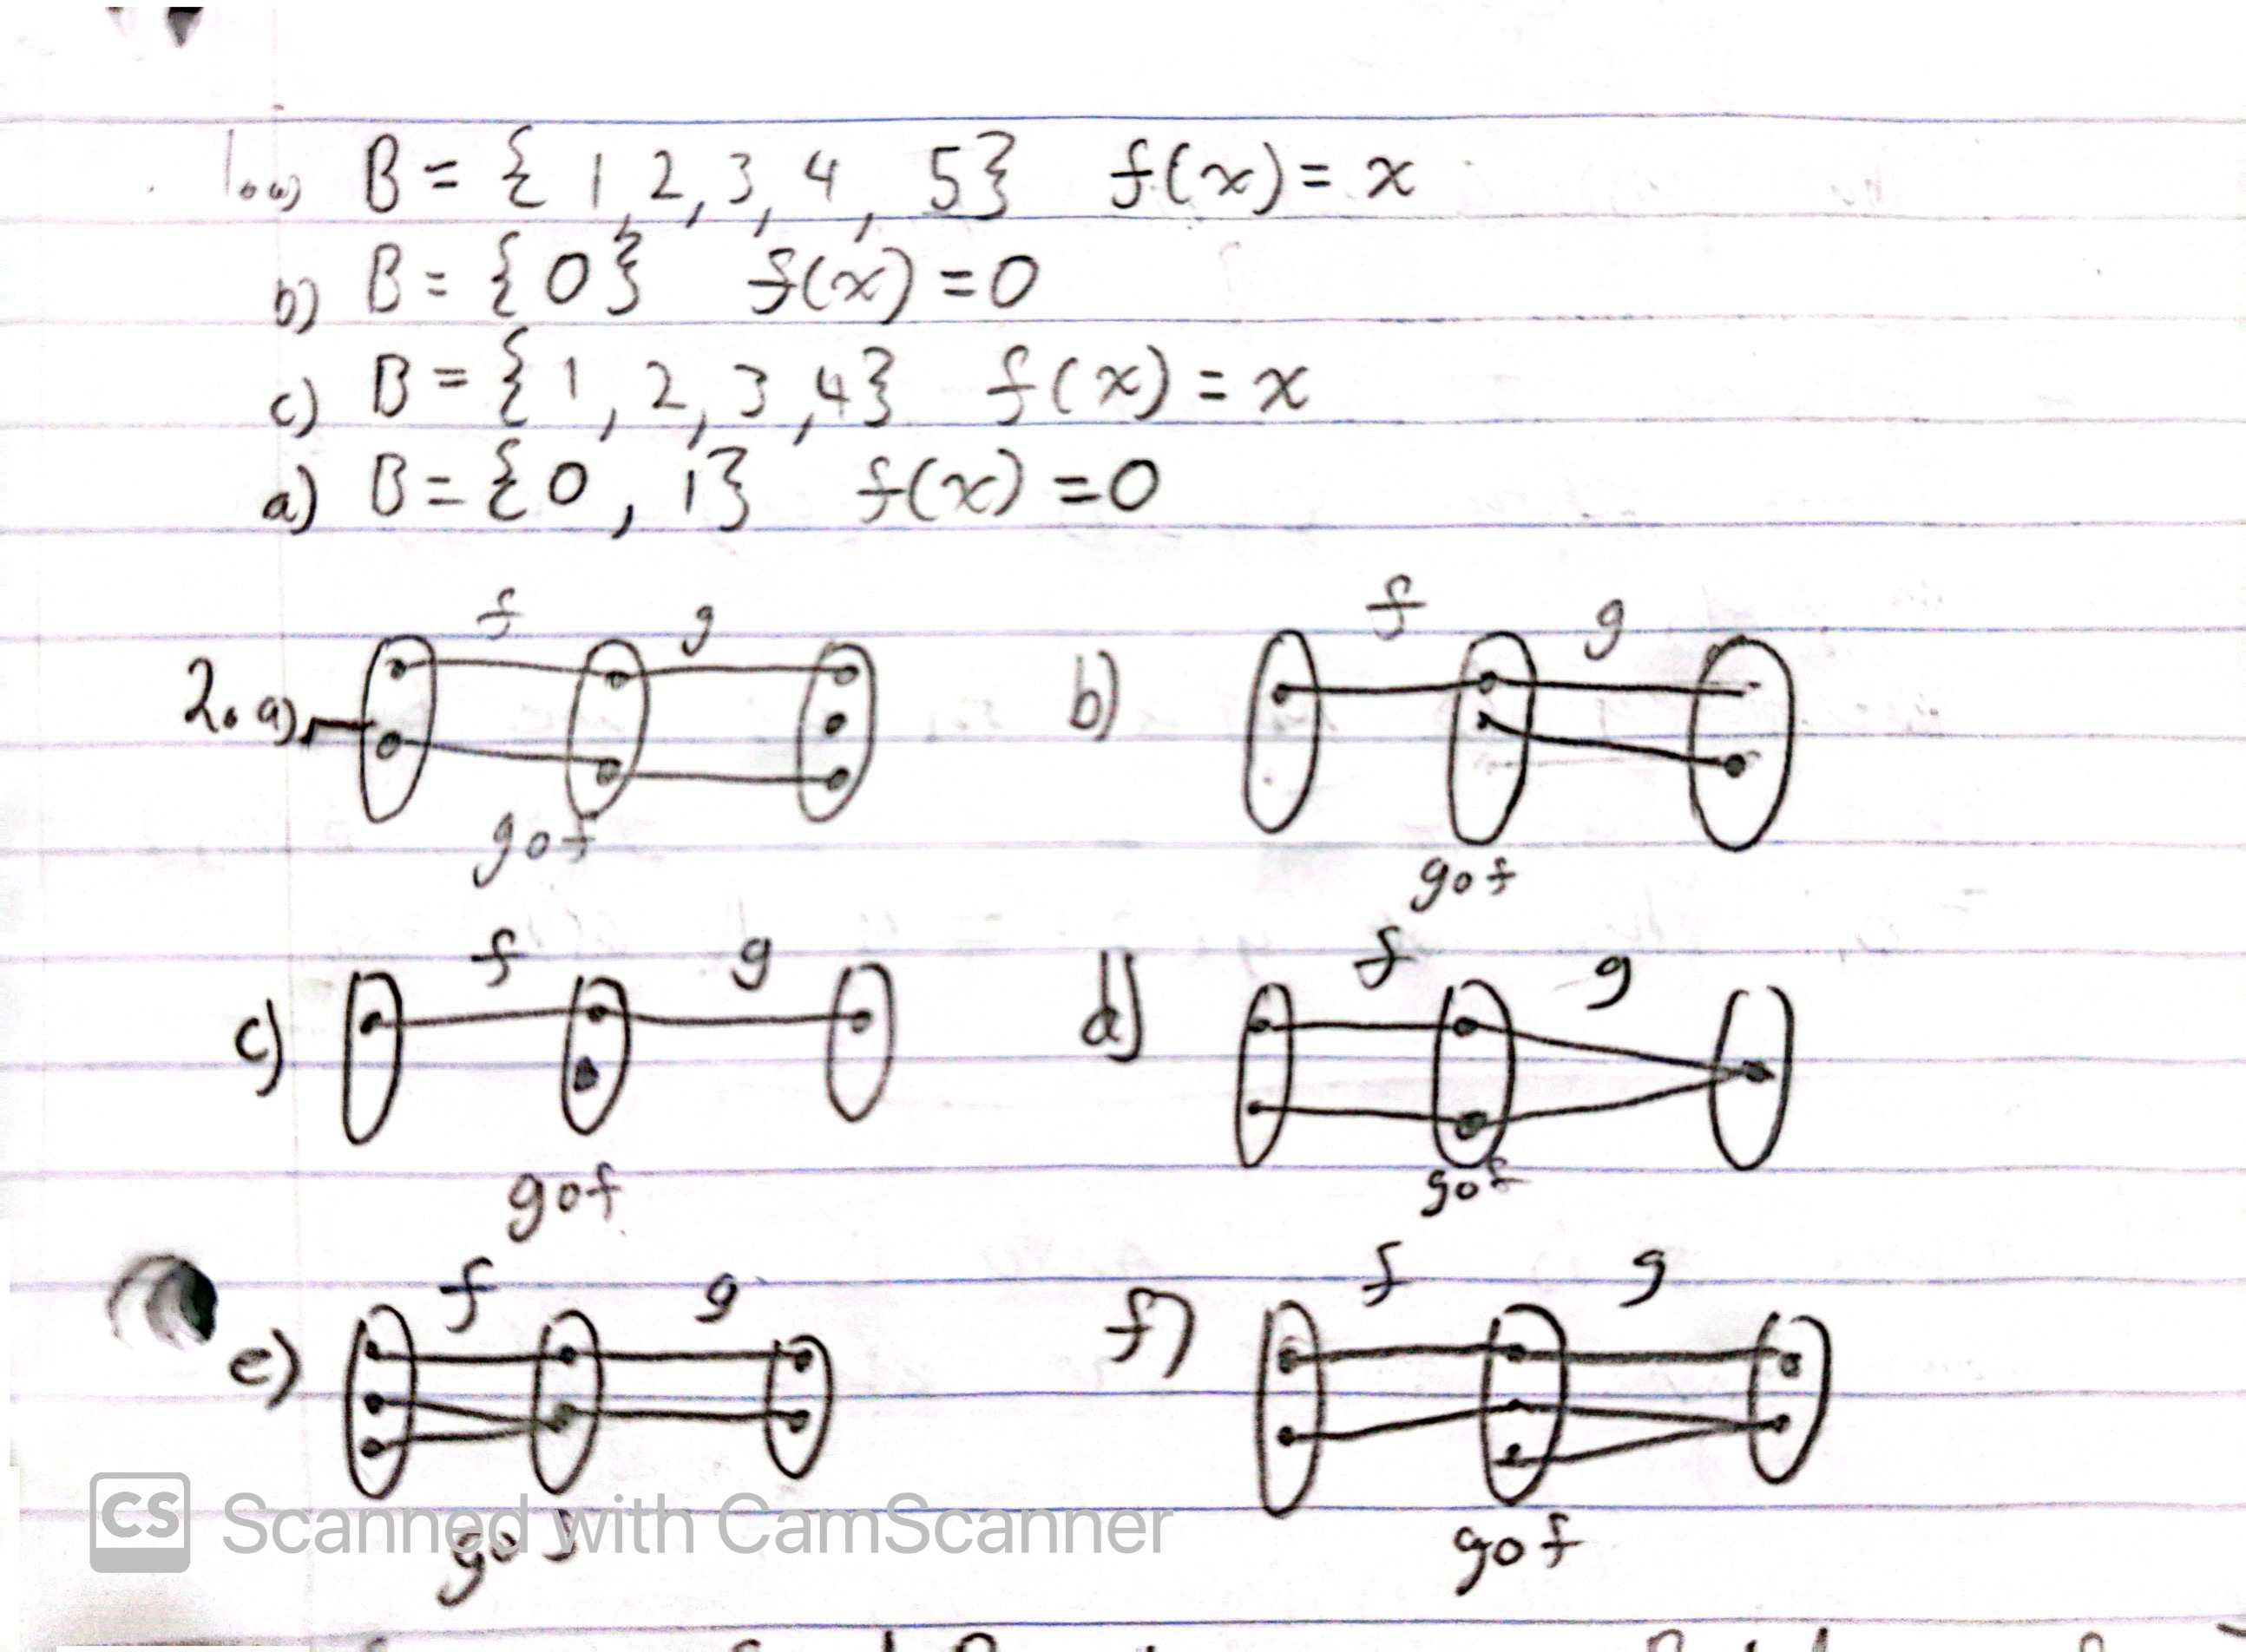
\includegraphics[scale=.1]{IMG_2640.JPG}
    \item [3] - \begin{itemize}
        \item Proof by contradiction: Assume that $f$ is not one to one.
        \item Then there exists $a_1$ and $a_2$ in $A$ where $a_1 \neq a_2$ but $f(a_1) = f(a_2)$ 
        \item This is impossible as we know that there exists a function $g$ where $g \circ f = I_a$. Since $I_a$ is a function which takes in $a$ and returns $a$, there cannot be a function $g$ which can take in one input and return 2 outputs. 
        \item $f(a_1) = f(a_2) =b$, then it is impossible for $g(b) = a_1$ and $g(b) = a_2$ as we expect $g \circ f = I_a$ but that means $g$ is not a function showing a contradiction 
        \item This means that $f$ must be one to one
    \end{itemize}
    \item [4] - \begin{itemize}
        \item Proof by contradiction: Assume that $f$ is not onto B
        \item Then there exists an element in B where it cannot be mapped from an element in A. 
        \item This is impossible as it is given that $f \circ g = I_b$
        \item $I_b$ is a function that maps $b$ to $b$ and if there is an element in A that doesnt map to B (this is the definiton of something not onto) then $g$ is not defined for all of $B$, making it not a function and providing a contradiction. 
    \end{itemize}
\end{itemize}

\end{document}